%! suppress = MissingLabel
\documentclass[11pt]{article}

% Packages
\usepackage{amsmath}
\usepackage{float}
\usepackage{graphicx}
\usepackage{sidenotes}
\usepackage[a4paper,
innermargin=2cm,
textwidth=12cm,
marginparwidth=5cm,
marginparsep=1cm,
heightrounded,
]{geometry}
\usepackage{etoolbox}
\usepackage{setspace}
\AtBeginEnvironment{quote}{\singlespacing\small}

\let\oldemph\emph
\renewcommand{\emph}[1]{\oldemph{\textbf{#1}}\marginpar{\textbf{#1}}}


%% Draw line
\usepackage{tikzpagenodes}

\usepackage{atbegshi}
\usepackage{csquotes}

\def\drawcode{%
\tikz [remember picture, overlay] \draw
([xshift=.5cm]current page text area.north east)
--
([xshift=.5cm]current page text area.south east);}

\AtBeginDocument{% For the first page
\drawcode}

\AtBeginShipout{% For the remaining pages
\drawcode}

% Document
\begin{document}
    \section{Introduction}

    \emph{Gartner Hype Cycle}:
    \begin{itemize}
        \item \emph{Innovation trigger} future, commercial value unknown
        \item \emph{Peak of inflated expection} specific success stories with a lot of restrictions
        \item \emph{Through of Disillusionment} understanding of limitations of technology
        \item \emph{Slope of Enlightment} use understanding to develop commercially viable usage
        \item \emph{Plateau of Productivity} technology becomes mainstream
    \end{itemize}

    \begin{figure}[H]
        \centering
        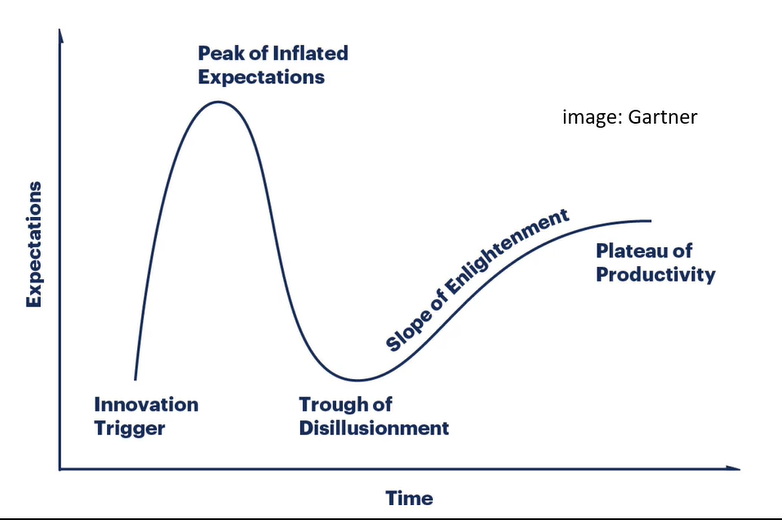
\includegraphics[width=0.8\textwidth]{img/hype.png}
        \caption{Hype}
        \label{fig:hype}
    \end{figure}

    \begin{figure}[H]
        \centering
        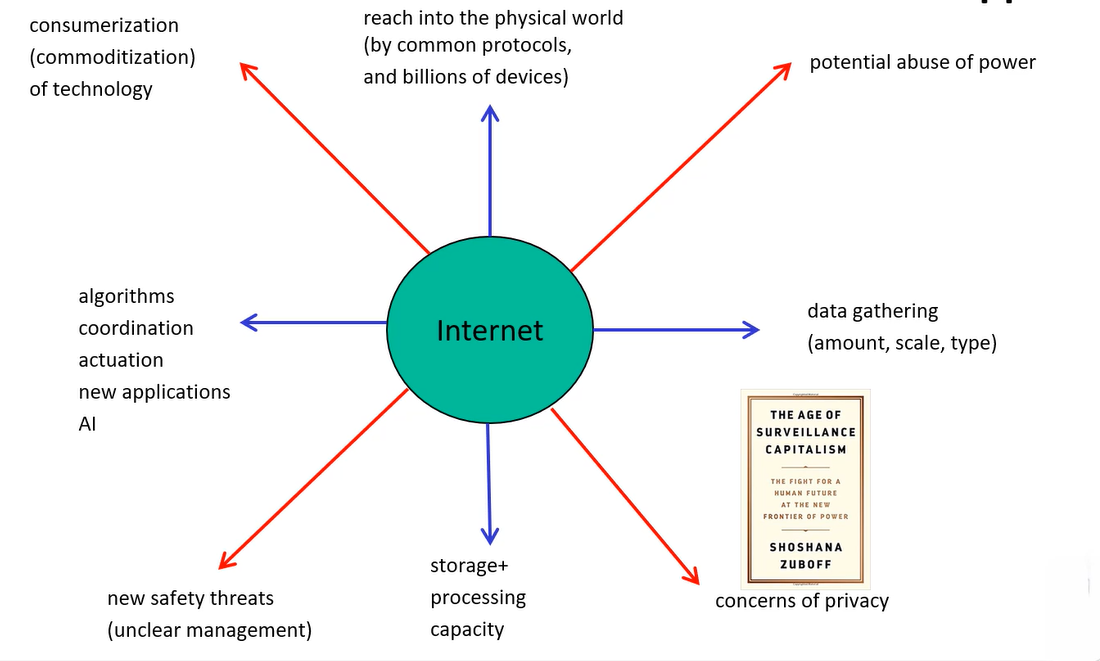
\includegraphics[width=0.8\textwidth]{img/internet.png}
        \caption{Internet}
        \label{fig:internet}
    \end{figure}

    Mainly focus on blue arrows in Fig~\ref{fig:internet}.

    \section{Examples}

    \subsection{Monitoring Energy Use example}

    \paragraph{Schematic}
    \begin{itemize}
        \item Red: direct data
        \item Red dotted: indirect data
        \item Blue: direct control
        \item Blue dotted: indirect control
    \end{itemize}

    \paragraph{Transformer}
    Report transformer data.
    \paragraph{Raspberry Pi}
    Create and provide overview report.
    Store data from smart meter.
    \paragraph{Smart meter}
    Report metering data.

    \paragraph{Questions}
    Which management concerns, where do we find management functionality, which quality concerns, who owns the data,
    what interests are there in the data, who controls the data, what are the `things'?

    \paragraph{3 tier architecture}
    UI, application, database.
    Many websites work like this.

    Architecture alternatives are obtained by different deployment choices of storing components on client machine and server machine.

    \paragraph{Integration}
    The system is composed of subsystems.
    Integration is at the network level.

    \paragraph{Data}
    \emph{Vertical analytics}:
    Data can be used to analyze processes in a home.

    \emph{Horizontal analytics}:
    Multiple homes can be monitored to learn about general things such as energy use, possibly using classification.

    \subsection{Quantified self}
    For proper horizontal analytics, not only monitor sick people, but also healthy people.

    \emph{Short cycle}:
    a standalone system that utilizes only the data of the individual.

    \begin{figure}[H]
        \centering
        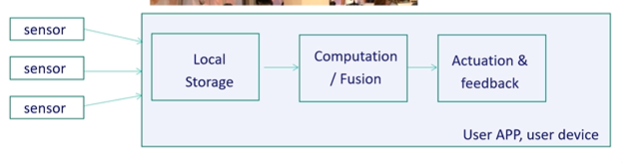
\includegraphics[width=0.8\textwidth]{img/short-cycle.png}
        \caption{Short cycle}
        \label{fig:sc}
    \end{figure}

    \emph{Long cycle}:
    employs a global storage of many users data, and horizontal analysis on that data.

    \begin{figure}[H]
        \centering
        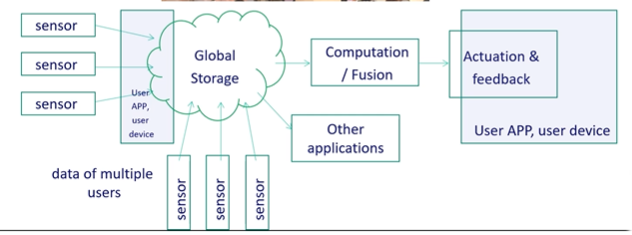
\includegraphics[width=0.8\textwidth]{img/long-cycle.png}
        \caption{Long cycle}
        \label{fig:lc}
    \end{figure}

    \emph{Alignment of platform owner and user}:
    user's interest is a personal outcome, and control over her own data.
    Platfor owner wants as much data as possible, obtain deep insight and market dominance.

    \section{Overview}

    \subsection{Definitions}

    Oxford \emph{IoT definition}:
    \begin{quote}
        Is the interconnection via the Internet of computing devices embedded in everyday objects, enabling them to send and receive data.
    \end{quote}

    Variety of definitions available, due to differences in scope (see p.3 of slides).
    We say: IoT = identifiable devices (attached to objects) and interconnected networks.

    \emph{Similar to internet}, but the IoT consists of devices
    \begin{itemize}
        \item with limited functions
        \item connected to low capacity networks
        \item without proper UI
        \item in large numbers (not just one-to-one)
        \item that interact with the real world
    \end{itemize}

    \paragraph{Scope}

    \begin{figure}[H]
        \centering
        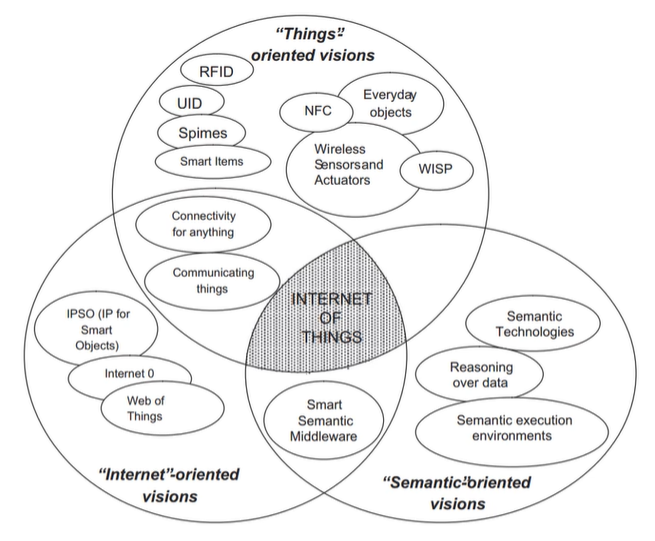
\includegraphics[width=0.8\textwidth]{img/paste-20201111123232.png}
    \end{figure}

    \emph{Cyber physical systems}: tight integration of communication, computation, physical world.

    \emph{Cloud computing}: build powerful services and applications on top of massive amounts of data, collected through embedded devices.

    IoT system consists of:
    \begin{itemize}
        \item Constrained devices (memory, processing power, energy, accessibility)
        \item Constrained networks (bitrate, packet loss, asymmetric links, etc)
        \item \emph{Internet services}: deal with large amounts of data and support processing
    \end{itemize}

    \subsection{Understanding IoT systems}
    \begin{itemize}
        \item Domains
        \item Architecture
        \item Communication stack and protocols
        \item Lifecycles of devices, services, applications
    \end{itemize}

    \section{Life Cycles}
    What is the life cycle of IoT systems and components and impact of application domain?

    \emph{Life cycle}:
    \begin{quote}
        The life cycle of a product or system is the series of stages it goes through from inception to decline.
    \end{quote}

    Typical: analysis, design, implementation, testing, maintenance, repeat.
    Life cycles for IoT pertain to devices, services and applications.
    Because, IoT applications are networked, which means the system is distributed and deployment and commisioning are cumbersome.
    Life cycles differ per domain.
    Lice cycle stages have typical use cases, and are key to understanding IoT architectural requirements.

    \begin{figure}[H]
        \centering
        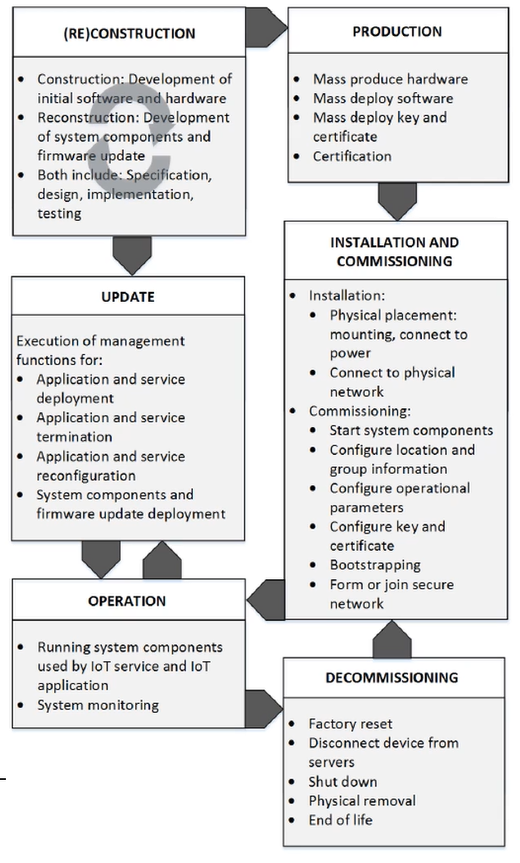
\includegraphics[width=0.8\textwidth]{img/paste-20201111124953.png}
        \caption{IoT device life cycle}
    \end{figure}

    Important: responsibilities and control of all stakeholders involved.

    Involved software types:
    \begin{itemize}
        \item Embedded operating system
        \item Libraries
        \item Components exposing services
        \item Applications
    \end{itemize}

    Software update packaging
    \begin{itemize}
        \item \emph{Firmware}: OS and middleware
        \item \emph{Module}: library/application
        \item \emph{Setting}: parameter setting
    \end{itemize}

    \begin{figure}[H]
        \centering
        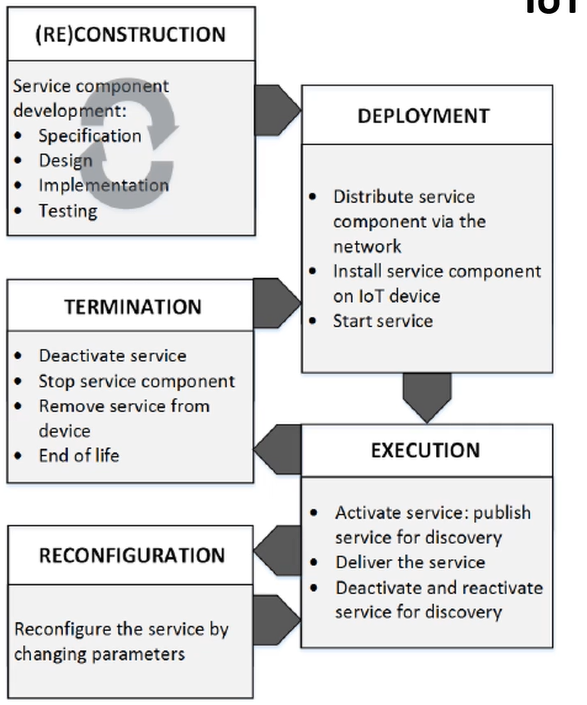
\includegraphics[width=0.8\textwidth]{img/paste-20201111125632.png}
        \caption{IoT service and component life cycle}
    \end{figure}

    \begin{figure}[H]
        \centering
        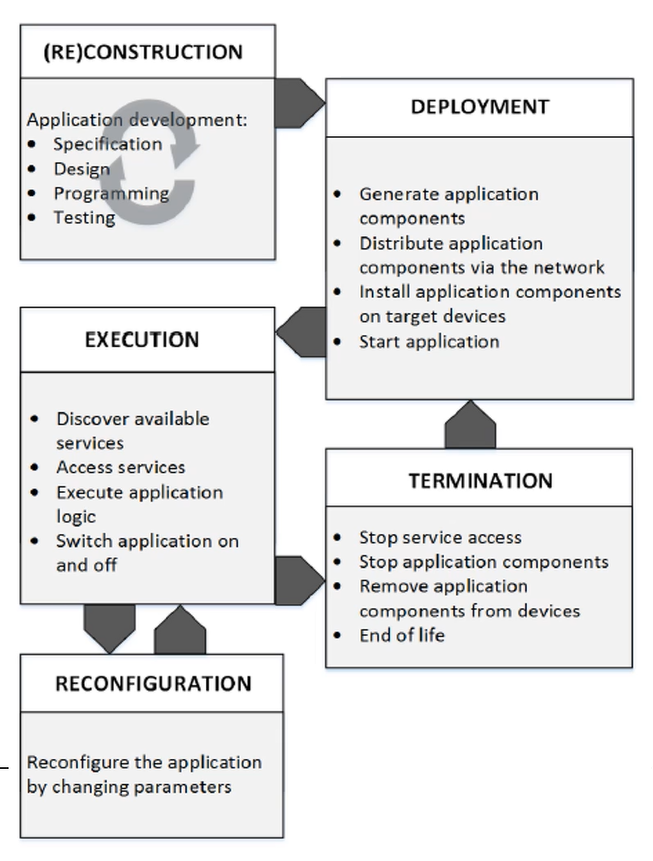
\includegraphics[width=0.8\textwidth]{img/paste-20201111125919.png}
        \caption{IoT application life cycle}
    \end{figure}

    Application life cycle depends on lice cycles of components and libraries (services).

    Extrafunctional properties:
    \begin{itemize}
        \item Security: trust new devices/components, access control, encryption, security management.
        \item Reliability, availability, safety: self monitoring
        \item Privacy: control on personal information
    \end{itemize}

    \paragraph{Characteristics of the home domain}
    The home is in principle unmanaged: one-time configuration, responsibility for software updates not assigned, problems/side effects very difficult to understand.

    \paragraph{Need for control function}
    Home needs more integration and brains: no gateway for everything, better network and equipment management, storage of history and persistent state, machine learning, etc.
    Use e.g.\ digital assistant (Google Assistant, Alexa, etc.)

    \paragraph{Characteristics of the office domain}
    The office is managed: central access control, clear procedures and responsibilities for system updates, standardization, higher cost acceptable.
    Conclicting concerns: bring your own device, data management.

    Other domains (city, industry) have further characteristics, have very implementation of lice cyles, and have different problems in life cycles.

    \section{Architecture}

    \subsection{Standards and platforms}
    Involved bodies and frameworks:
    \begin{itemize}
        \item ETSI (network)
        \item ITU (network)
        \item IETF (protocols)
        \item EU projects such as IoT-A, SENSEI for books and architectures
        \item OSG (data, information)
        \item OMA (Open mobile alliance)
        \item IEEE (protocols)
    \end{itemize}

    The war on standards,
    like Apple HomeKit, Google Home with Google Assistant, Microsoft with Azure IoT, Amazon with AWS IoT, Philips with HUE, etc.

    \subsection{Architecture}

    \begin{figure}[H]
        \centering
        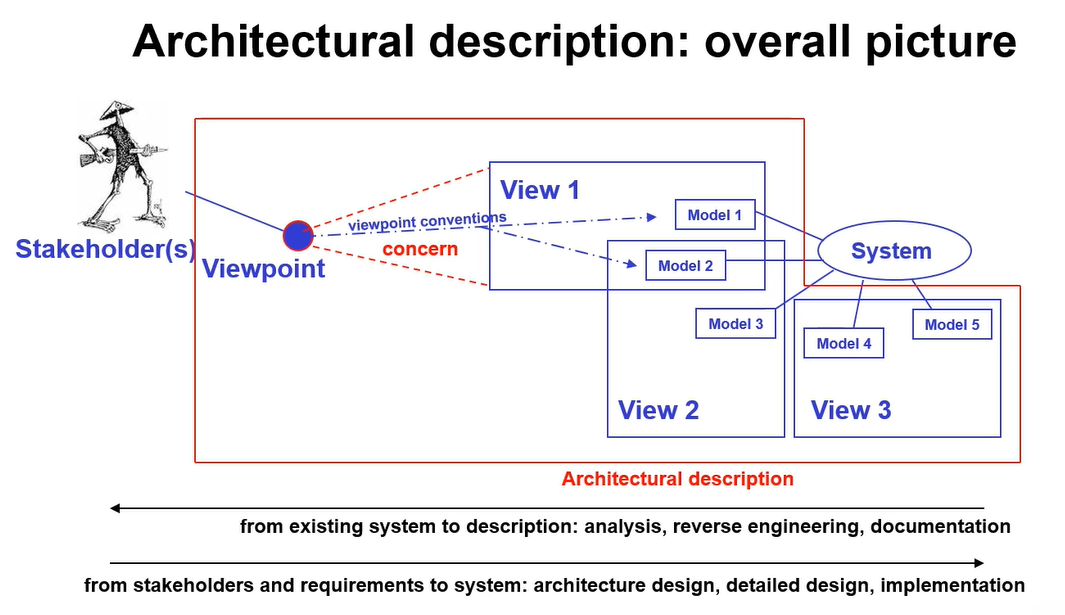
\includegraphics[width=0.8\textwidth]{img/paste-20201111132026.png}
        \caption{Architectural description}
    \end{figure}

    A collection of models organized into views that examine a system from a certain viewpoint defined by the concern of a stakeholder.
    For understanding, andalysis, communication, construction, documentation.

    \emph{Architecture definition}
    \begin{figure}[H]
        \centering
        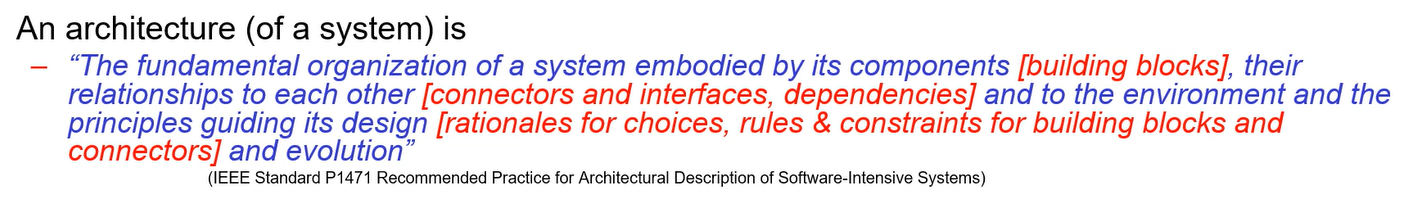
\includegraphics[width=0.8\textwidth]{img/paste-20201111132140.png}
        \caption{Architecture definition}
    \end{figure}

    Views and models:
    \begin{itemize}
        \item Logical layering/technical views: overall impression
        \item Deployment/physical view: organizational alternatives
        \item Development view: organization of software
        \item Process view: operation and interoperation, protocols, architectural patterns
        \item Data view: data semantics, protection, etc
    \end{itemize}

    \begin{figure}[H]
        \centering
        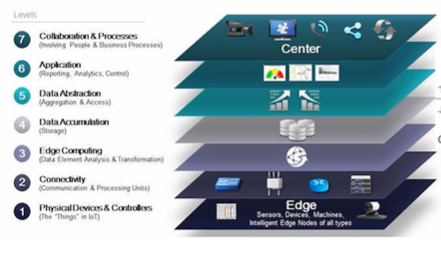
\includegraphics[width=0.8\textwidth]{img/stack.png}
        \caption{Reference model for IoT}
    \end{figure}

    \subsection{Deployment view}

    Physical elements
    \begin{itemize}
        \item `Things': Low capacity devices with sensors, actuators and an identifier
        \item Infra structure: switches, routers (connectivity with network technology), gateways (converting between parties, different layers of OsI stack), networks
        \item Storage devices
        \item User devices; phones, tablets, etc
        \item Embedded devices
        \item `Fog'; high capacity devices in the vicinity of data generation
        \item `Clouds': massive storage and execution power
    \end{itemize}

    Mapping IoT Arch. elements to devices, balance the following:
    \begin{itemize}
        \item Functional: sensing, actuating, application logic, communication, storage, data information, management
        \item Extra functional: dependability, performance, QoS, resource management, interoperability, mobility, ownership
        \item Boundary conditions: distributed systems, given components and protocols, network standards, legal matters
    \end{itemize}
    Think about \emph{Reliability vs. availability} and \emph{Security vs. privacy}

    \paragraph{Analytics}
    \emph{Vertical analytics}: Data from single unit.
    \emph{Horizontal analytics}: Data from many units.

    \paragraph{Managerial domain}
    Extra-functional domain, control span of a managing stakeholder.
    \emph{Physical managerial domain}: defined by physical access to domain and networks.
    \emph{Logical managerial domain}: Control over software elements and data.
    Derived from physical domain.

    Types of managerial control:
    \emph{Life cycle control}: Control over actions in life cycle like switching on/off.
    \emph{Behavioral control}: Controlling the behavior of a device or software element when it `runs'.

    \paragraph{Architecture alternatives}
    Take into account life cycles of devices/services/applications, and requirements set by all stakeholders.
    Architecture/deployment decisions and views are obtained from scenarios.
    \begin{itemize}
        \item Integration: put functions together on one device
        \item Distribution: put functions on different devices
        \item Virtualization: decoupling of logical and physical representation
        Improves simplicity, generalization, flexibility, cost, lower performance.
t    \end{itemize}

    Depends on location, form factor, numbers, energy, cost, system complexity, component availability, software/framework availability.


    \paragraph{Communication}
    Direct communication between communicating parties over a comm. protocol that they together implement.

    Reduces latency.

    Indirect:
    \begin{itemize}
        \item \emph{Broker}: A component that handles and translates calls between two or more parties.
        \item \emph{Proxy}: A component that acts on behalf of another component, implementing the same interface, and sometimes caching.
        \item \emph{Store}: One component leaves data and another one picks it up.
    \end{itemize}
    Reduces dependencies between parties, w.r.t. time and space.

    \begin{itemize}
        \item \emph{Push}: Control flow and data go in same direction (`call-back', `event driven').
        Reduces latency, needs administration at sender.
        \item \emph{Pull}: Control flow and data go in opposite direction (`call', `polling')
        Obtain data when required, increases latency.
    \end{itemize}

    \paragraph{Data}
    Data storage and handling determined by privacy concerns, need for collecting evidence, cost concerns, value of data.

    \paragraph{Application and control logic}
    Location of application logic and ocntrol logic depends on privacy concerns, latency requirements, used framework, performance, complexity.

    See p. 35 in slides for a summery of all options and their consequences on requirements.

    \subsection{Privacy, safety and security}
    \begin{itemize}
        \item \emph{Privacy}: control over personal information.
        \item \emph{Safety}: Freedom from danger or risk on injury resulting from recognized but potentially hazardous events.
        \item \emph{Security}: Regulating access to assets according to some policy.
    \end{itemize}

    \subsection{Reference model}
    \emph{Reference model} defines generically what binds architectures (?) together:
    \begin{itemize}
        \item \emph{Domain model}: relevant concepts and relations in IoT
        \item \emph{Information model}: data structures of the domain model elements
        \item \emph{Functional model}: (generic) operations
        \item \emph{Communication model}: communication interactions between entities
    \end{itemize}

    \emph{Reference architecture}: an architecture description that takes this reference model as starting point.

    Concerns and objectives:
    \begin{itemize}
        \item Re-use resources across application domains
        \item A set of support services
        \item Different abstraction levels
        \item Sensing and actuating can assume roles in different applications
        \item Trust, security, privacy, safety
        \item Include different service delivery models
        \item Simple integration/management
        \item Life cycle support
    \end{itemize}

    \section{The Things}

    \paragraph{Resource limitations}
    \begin{itemize}
    \item Memory: available flash and RAM
    \item Processor: Mhz, instruction set, address width, power management
    \item Communication: transceiver power, bps, protocol complexity
    \item Energy: available joules and how they are replenished
    \end{itemize}

    \paragraph{Device classifications}
    Three classes representing memory limitations:
    \begin{itemize}
        \item C0: dependent on proxies for secure internet inclusion
        \item C1: only low resource protocols
        \item C2: can run most internet protocols
    \end{itemize}

    \begin{figure}[H]
        \centering
        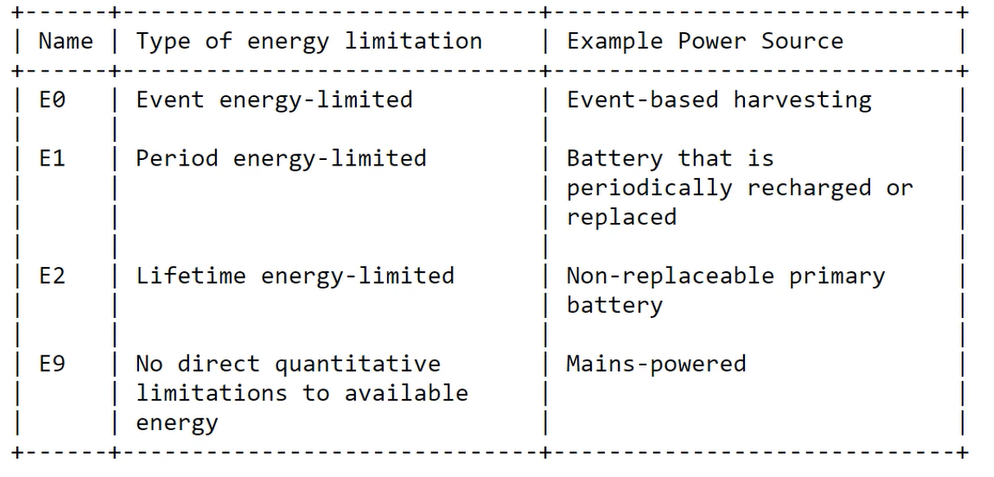
\includegraphics[width=0.8\textwidth]{img/paste-20201117123757.png}
    \end{figure}

    \begin{figure}[H]
        \centering
        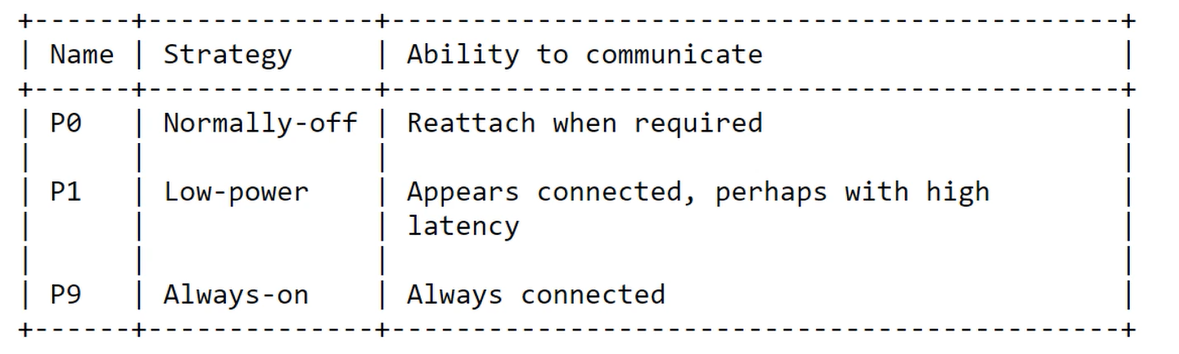
\includegraphics[width=0.8\textwidth]{img/paste-20201117123806.png}
    \end{figure}

    \begin{figure}[H]
        \centering
        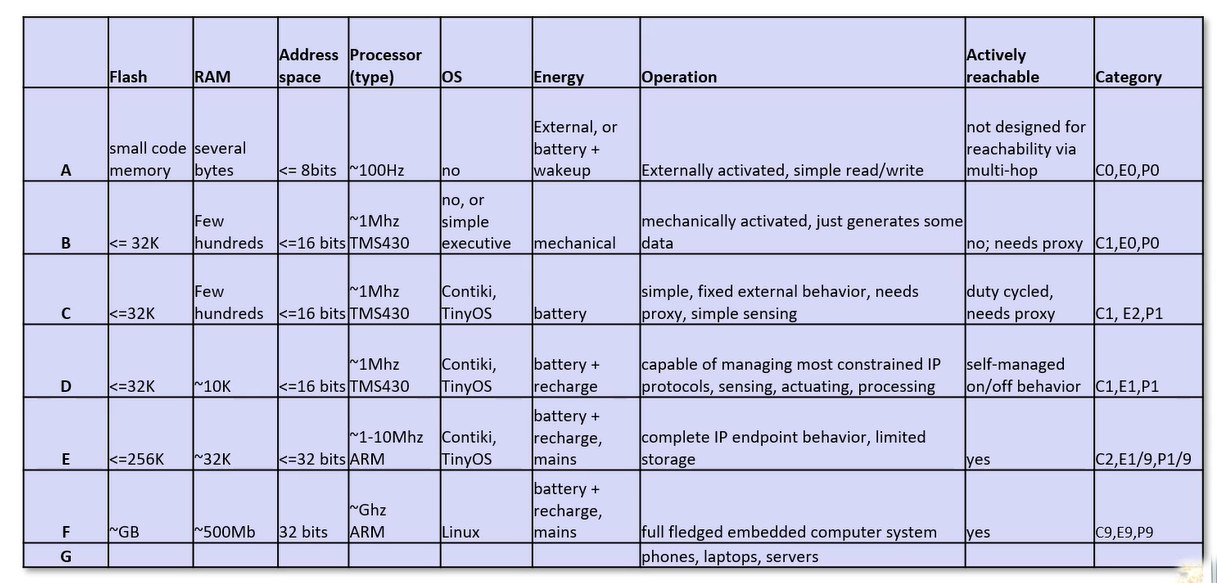
\includegraphics[width=0.8\textwidth]{img/paste-20201117124401.png}
    \end{figure}

    \paragraph{Concerns and management}
    Can it
    \begin{itemize}
        \item join a network?
        \item be configured?
        \item be updated (over the air)?
        \item run IP?
        \item secure itself?
    \end{itemize}

    \subsection{What is new in IoT}
    \begin{itemize}
        \item
        There are \emph{many} things.
        \begin{itemize}
            \item
            We have \#things / person $>>$ 1.
            \item Connected/talk to each other
            \item
            Autonomy of things;
            self management and self healing.
            \item
            Scalability: many things sharing your wireless LAN.
        \end{itemize}
        \item
        Things have limitations
        \begin{itemize}
            \item low processing power
            \item memory
            \item low capacity network
            \item battery operated
            \item embedded: no UI
        \end{itemize}
        \item
        Enable new applications because of the large number of things and far-reaching locations.
        \item
        Scale and locations come with complex concerns; every IoT device is very different.
    \end{itemize}

    \paragraph{WSN vs. IoT vs. M2M}
    IoT:
    \begin{itemize}
        \item System

        is platform, open, extensible, interoperable
        \item Protocol

        IP and higher to endpoints and on top of low resource networks
        \item Applications

        Use IP protocols and developed seperately
        \item Management

        Explicit, use IP management protocols.
    \end{itemize}
    WSN:
    \begin{itemize}
        \item System

        .. is the application: built with a specific application
        \item Protocol

        application oriented
        \item Applications

        Developed and optimized along with entire system
        \item Management

        Implicit, part of application.
    \end{itemize}
    M2M:
    \begin{itemize}
        \item System

        .. is the application, closed.
        \item Protocol

        standardized, for low-resource networks.
        \item Applications

        Classes, developed and optimized along with entire system.
        \item Management

        Explicit, built into protocols.
    \end{itemize}

    \section{Networks}


    \subsection{Physical organization}

    General architecture:
    \begin{itemize}
        \item Moving clusters of nodes with sensing capability
        \item Static ambient nodes attaching to clusters
        \item IP-based network with wide-area coverage
    \end{itemize}

    \begin{figure}[H]
        \centering
        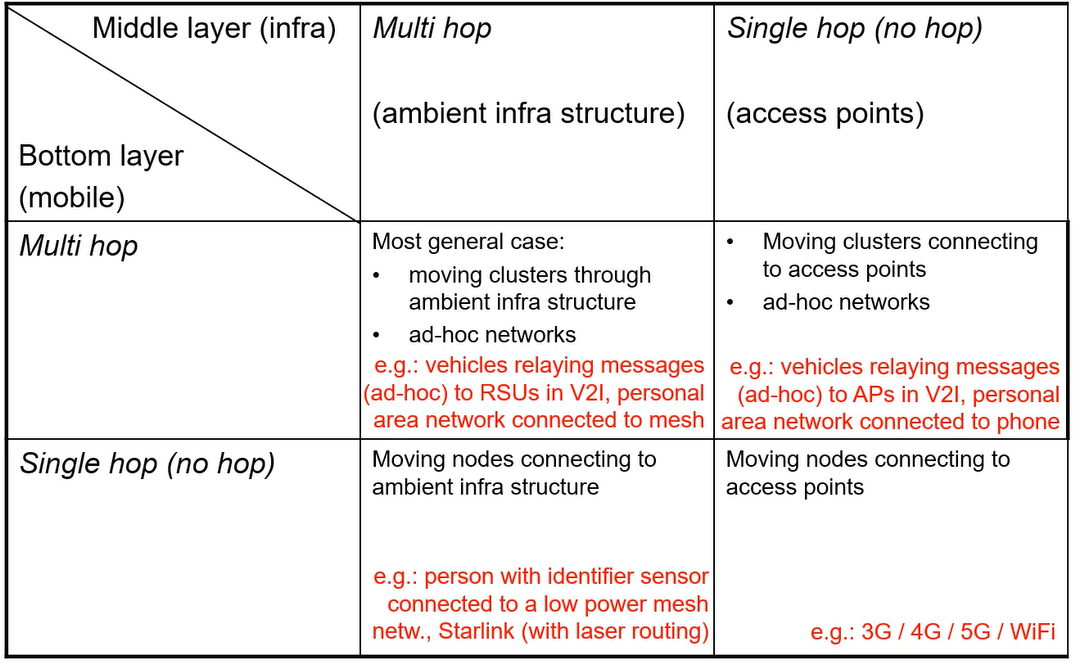
\includegraphics[width=0.8\textwidth]{img/paste-20201208121214.png}
    \end{figure}

    \subsection{Internet Protocol}

    \begin{itemize}
        \item Physical:  send bits on medium
        \item MAC: managing medium access
        \item Network: sender to receiver/routing
        \item Transport: break messages into packets, delivery guarantees
        \item Session, Presentation, Application merged in one application layer for Internet Protocol
    \end{itemize}

    \emph{Hourglass of IP}: a unified protocol and naming scheme to enable communication between any pair of devices (diverse physical layers -> ip -> diverse applications).

    \emph{Essence of IoT}: a unified protocol and naming scheme to enable communication between any pair of things.

    Setback: IP endpoints should always be active and reachable.
    Devices cannot always guarantee this; passive nodes/batery-less nodes/duty cycling etc.
    We need technology to solve this (gateways).

    \subsection{IEEE local area networks}

    Network approaches:
    \begin{itemize}
        \item Physical neighbors: shared medium or point-to-point
        \item Switching: layer two
        \item Connecting networks: layer 3
        \item Packet oriented
        \item Full network: full connectivity
    \end{itemize}

    Wired: nodes can be powered through network, difficult to scale.

    Wireless: typical for really large numbers, inherently unreliable medium.

    See slides for an overview of different IEEE 802 groups.

    \subsection{Medium sharing}

    \emph{Shared medium}: can be a wire/bus but also wireless connection.

    Techniques applied for wireless:
    \begin{itemize}
        \item FDMA: multiple channels.
        \item TDMA: division in timeslots, introduces need for time synchronization

        Potentially wasteful when slots are not used.

        \item Master-slave
        \item CSMA: medium access protocols, uses channel assessment

        CSMA/CD, for wired: sense carrier, transmit and monitor for collisions (send jamming signal if another transmission comes in), complete transmission.

        CSMA/CR, for wired: sense carrier, transmit and monitor for collision (priority based choice), complete transmission.

        CSMA/CA, for wireless: transmission power is low, introduces need for collision avoidance instead of monitoring.
        Uses acknowledgement messages.

        Collisions due to unfortunate timing or due to hidden nodes.
        This can be solved using Request To Send signals.

        \item CDMA: concurrent access of the medium, due to coded packets, requires orthogonal codes

        \item \emph{Beacon}: periodic packet broadcasts, that enforce a globally slotte structure of the medium access.
        Can also be used for clock synchronization.
        See p. 35 for 802.11e example.
    \end{itemize}

    \subsection{Energy reduction}

    Techniques:
    \begin{itemize}
        \item Asymmetry: low-power nodes 1 hop away from well-powered infrastructure

        \item Trade connectivity for energy: control transceive power.
        \item Duty cycling

        We use strict time synchronization, or let sender send wakeup messages, or switc transceiver on sufficiently long to guarantee meeting the sender.

        \item Demand driven: event driven control of radio
        \item Push/pull: let low power partnet always take initiative (so that it never has to wait)

        Push/pull by node/environment.
        Solutions: aligh communication with periodic synchronization of the node with ints environment; provide always-on environment for demand driven radio control.

        \item Trade power for range and throughput.
    \end{itemize}

    \subsection{Wide area initiatives}

    Tradeoffs: communication range, data rate, transceiver power, spectrum usage.

    \emph{LoRaWAN}

    %TODO: figure

    LoRaWAN: star topology, uses Aloha Mac protocol, adaptive data rate managed by gateway.
    Three classes of devices.

    Services: geolocation and identification and security.


    \subsection{Metrics}

    \begin{itemize}
        \item Throughput: number of bytes per time unit
        \item Latency or delay: time difference in initiation of a transmission and the start of the receipt
        \item Jitter: variations in time
        \item Fairness: bound on delay in access to a transmission channel
        \item Overhead
        \item Scalability: as utilization or as dimensioning (scale number of gateways of LoRaWAN with number of low-power nodes)
        \item Predictability
        \item Reliability: resilience against interference
        \item Power
        \item Range
    \end{itemize}

    See p. 54 for table.

    \section{OpenAIS example}


    \subsection{Internet of Lights}

    \emph{Technology convergence}: Dumb to smart (e.g. mobile phones).

    \emph{Lightning system evolution}: on gartner scale, lightning systems are reaching the plateau of productivity

    Approaches:
    \begin{itemize}
        \item Cloud-based: excellent services, high latency, privacy concerns
        \item Edge-computing: poor services environment, low latency, good price
        \item OpenAIS: allows local controls, integration with cloud possible.
        OpenAIS is combination of cloud- and edge-based computing.
    \end{itemize}


    \emph{OpenAIS} is a standardization attempt for IoL (Internet of Light) vision.
    Light architecture for office buildings.

    Bullshit video die nergens over gaat, werd blijkbaar ook gebruikt in glow.

    \begin{figure}[H]
        \centering
        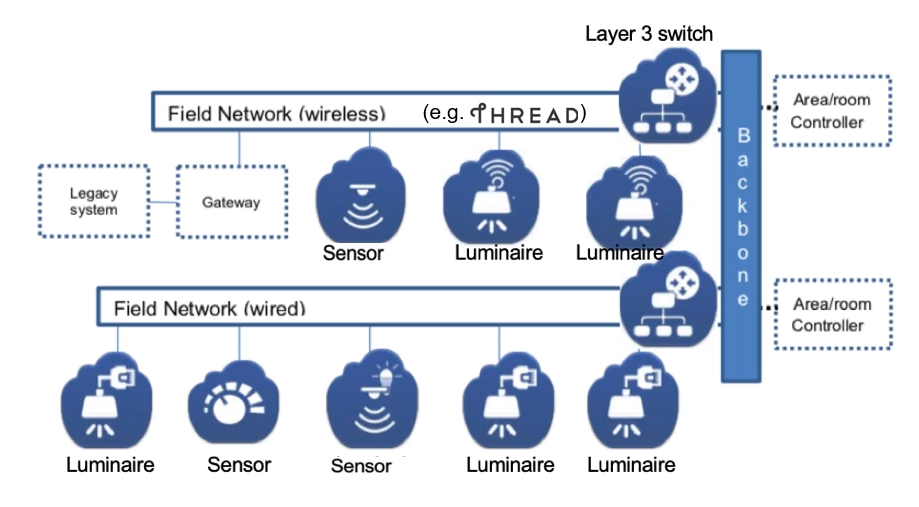
\includegraphics[width=0.8\textwidth]{img/paste-20201208141044.png}
    \end{figure}

    \emph{Gateway}: connect legacy networks to OpenAIS

    \emph{Luminaire}: device with one or more LED drivers

    \emph{Sensor}: device wiht only sensor on

    \emph{Area controller}: device with only computation and networking capabilities

    \emph{Routers and switches}: basic networking core

    More detailed view:
    \begin{figure}[H]
        \centering
        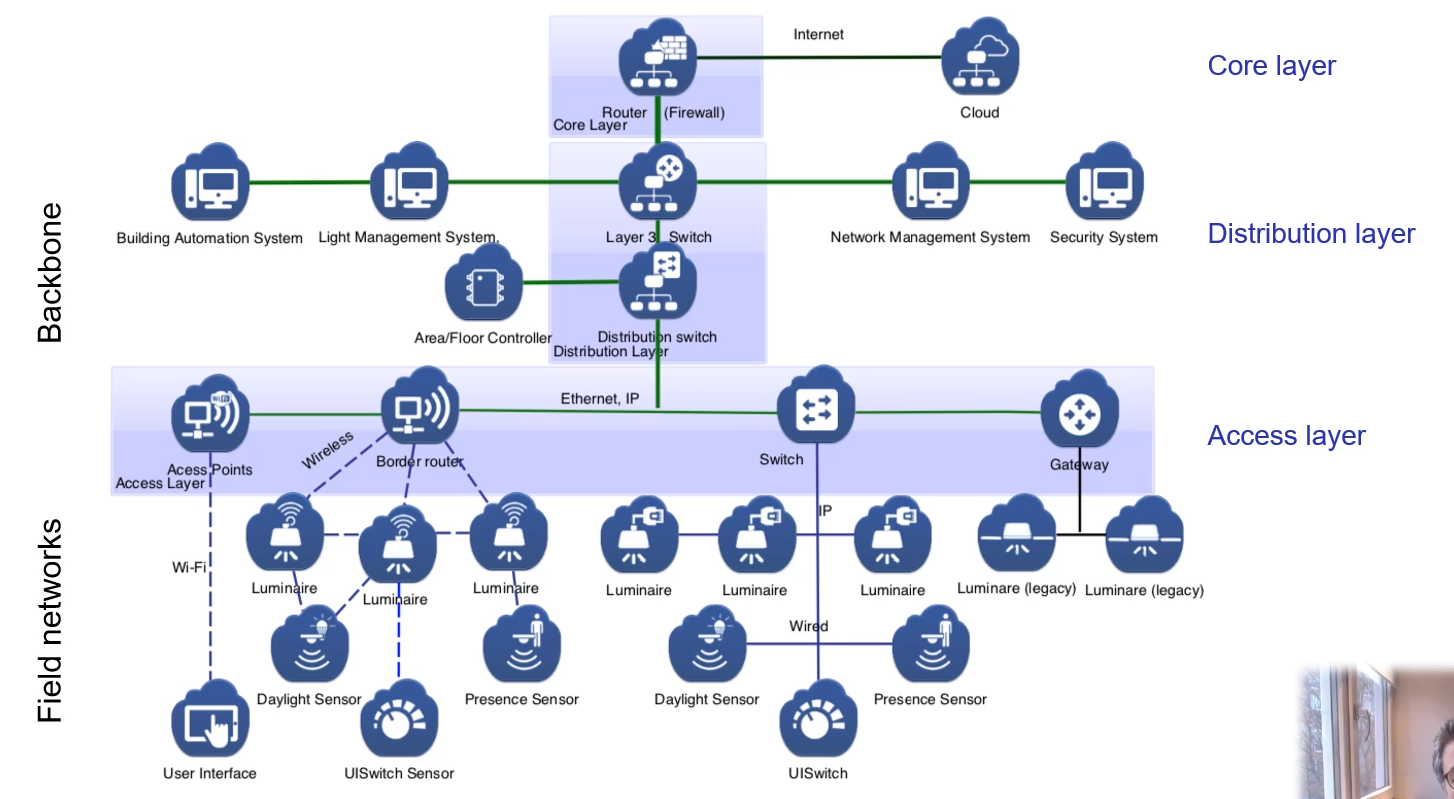
\includegraphics[width=0.8\textwidth]{img/paste-20201208141151.png}
    \end{figure}

    \emph{OpenAIS device classes}
    \begin{itemize}
        \item \emph{Low resource devices}: low power cpu, limited OS, etc.
        \item \emph{Medium resource devices}: standard embedded device with on-chip flash and RAM, real time kernel
        \item \emph{Full resource devices}: standard OS like Linux, state of the art CPU, external RAM
    \end{itemize}

    \emph{Application layer functions}: high level functionality needed for lightning, and gateway for unified behavior.
    \begin{itemize}
        \item Sense: detect changes in environment
        \item Actuate:
        \item Control: implement lightning algorithm
        \item DataCollect: collect data from sensors etc
        \item Group:
        \item Scene: specific scenarios
        \item Gateway: legacy systems
    \end{itemize}

    \emph{Infrastructure layer functions}: these functions take care of low level platform services.
    \begin{itemize}
        \item Application layer function
        \item Discover
        \item Communication
        \item Update
        \item Security
        \item Configuration
        \item DeviceContainer
    \end{itemize}

    OpenAIS uses the \emph{Sensor-Controller-Actuator} model
    \begin{figure}[H]
        \centering
        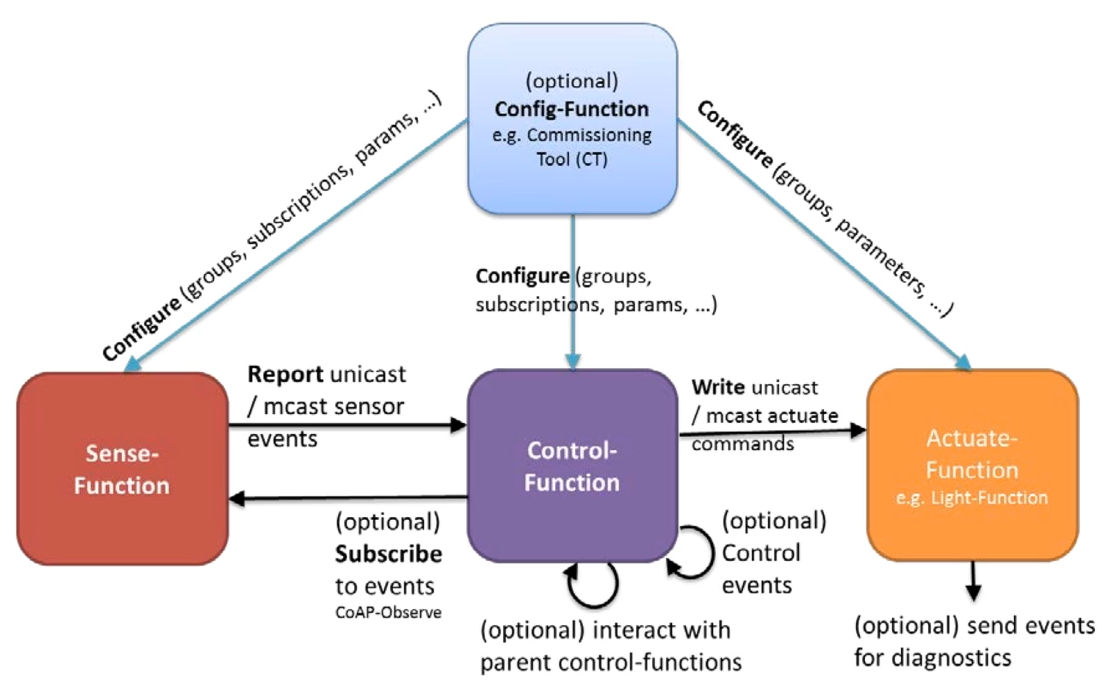
\includegraphics[width=0.8\textwidth]{img/paste-20201208141824.png}
    \end{figure}

    \emph{Function interfaces}
    \begin{itemize}
        \item IControl
        \item IData
        \item IConfig
        \item IDiscover
    \end{itemize}

    \emph{Control function}s give flexible distribution of control.
    \emph{Control stacking}: control functions may be stacked, leading to different levels of control.
    E.g.\ external energy management: max 60\% brightness sent to other controllers.

    \emph{LWM2M} secure direct unicast communication between field devices.

    \emph{Low power radio access point}: provides access to a wireless IPv6 network that uses a low-power wireless protocol (by means of border router and linux host).

    \emph{Object data model}: illustrates sytem resources in a structured fashion.
    Resource and object definitions are described, together with default device behaviour relating to endpoint discovery etc.

    \emph{OpenAIS group}: formed by sharing a group vector.
    Variety of use cases, e.g.\ sensor shares data with relevant Objects.

    \emph{OpenAIs group communication (OGC)}
    Support the above.
    Allow multicast using OGC.
    OGC reliability: increased w.r.t IPv6 UDP multicast.


\end{document}
























